\documentclass[12pt]{article}
\usepackage[margin=2.5cm]{geometry}
\usepackage{enumerate}
\usepackage{amsfonts}
\usepackage{amsmath}
\usepackage{fancyhdr}
\usepackage{amsmath}
\usepackage{amssymb}
\usepackage{amsthm}
\usepackage{mdframed}
\usepackage{graphicx}
\usepackage{subcaption}
\usepackage{adjustbox}
\usepackage{listings}
\usepackage{xcolor}
\usepackage{booktabs}
\usepackage[utf]{kotex}

\definecolor{codegreen}{rgb}{0,0.6,0}
\definecolor{codegray}{rgb}{0.5,0.5,0.5}
\definecolor{codepurple}{rgb}{0.58,0,0.82}
\definecolor{backcolour}{rgb}{0.95,0.95,0.92}

\lstdefinestyle{mystyle}{
    backgroundcolor=\color{backcolour},
    commentstyle=\color{codegreen},
    keywordstyle=\color{magenta},
    numberstyle=\tiny\color{codegray},
    stringstyle=\color{codepurple},
    basicstyle=\ttfamily\footnotesize,
    breakatwhitespace=false,
    breaklines=true,
    captionpos=b,
    keepspaces=true,
    numbers=left,
    numbersep=5pt,
    showspaces=false,
    showstringspaces=false,
    showtabs=false,
    tabsize=1
}

\lstset{style=mystyle}

\pagestyle{fancy}
\renewcommand{\headrulewidth}{0.4pt}
\lhead{Hyungmo Gu}
\rhead{CSC209 Week 6 Notes}

\begin{document}
\title{CSC209 Week 6 Notes}
\author{Hyungmo Gu}
\maketitle

\section*{Struct 1 of 3}

\bigskip

\begin{itemize}
    \item Introducing Structs
    \begin{itemize}
        \item \textbf{struct/structures} is like dictionary in Python or object in Javascript
        \item there are differences between array and structure

        \begin{center}
        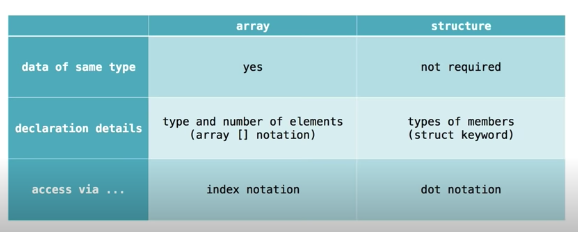
\includegraphics[width=\linewidth]{images/week_6_structs_1_1.png}
        \end{center}

        \item items in struct is called \textbf{member}
        \item items in array is called \textbf{element}
    \end{itemize}

    \bigskip

    \begin{lstlisting}[language=c,caption={struct\_example\_1.c}]
    #include <stdio.h>
    #include <string.h>

    int main() {
        struct student {
            char first_name[20];
            char last_name[20];
            int year;
            float gpa;
        };

        struct student good_student;

        strcpy(good_student.first_name, "Jo");
        strcpy(good_student.last_name, "Smith");
        good_student.year = 2;
        good_student.gpa = 3.2;

        printf("Name: %s %s\n", good_student.first_name, good_student.last_name);
        printf("Year %d. GPA %.2f\n", good_student.year, good_student.gpa);

        return 0;
    }
    \end{lstlisting}

\bigskip

\section*{Struct 2 of 3}

\bigskip

\begin{itemize}
    \item Using Structs in Functions
    \begin{itemize}
        \item Array pass function by \textbf{reference} (of the pointer of first element).
        \begin{itemize}
            \item Changing value inside affects outside
        \end{itemize}
        \item Struct pass function by \textbf{value} like int and string.

        \begin{itemize}
            \item Changing value in function doesn't affect value outside
            \item Pointer used to pass by \textbf{reference}

    \begin{lstlisting}[language=c,caption={struct\_example\_2.c}]
    #include <stdio.h>
    #include <string.h>

    struct student {
        ...
    };

    void change(struct student *s) { // <- passes by reference
        ...
    };

    int main(void) {
        struct student good_student;
        ...
        change(&good_student); // <- to pass function by reference (This is too cool!!!)
        ...
        return 0;
    }
    \end{lstlisting}
        \end{itemize}

    \end{itemize}
\end{itemize}

\end{itemize}


\bigskip

\section*{Struct 3 of 3}

\bigskip

\begin{itemize}
    \item Pointer to Structs
    \begin{itemize}
        \item \textit{(*p).student\_name} is hard to define, and read
        \item \textit{p-\textgreater student\_name} is the same as above, but easier to read.
        \begin{itemize}
            \item This is called \textbf{syntactic sugar}
        \end{itemize}
    \end{itemize}

    \begin{lstlisting}[language=c,caption={struct\_example\_3.c}]
    #include <stdio.h>
    #include <string.h>

    struct student {
        char first_name[20];
        char last_name[20];
        int year;
        float gpa;

    };

    int main(void) {
        struct student s;
        struct student *p;

        ...

        (*p).gpa = 3.0;
        p->year = 3; //<- HERE!!

        strcpy(p->first_name, "Hello");

        ...
        return 0;
    }
    \end{lstlisting}
\end{itemize}

\end{document}